%==============================================================================
%  Paper 6 (JOURNAL) - Federated Learning for Cross-Domain Network Intrusion
%  Detection: A Domain-Distance Study with a Leakage-Free Evaluation Protocol
%  and Adversarial Robustness Analysis on a Cloud Testbed.
%  Target venue: JOIN (Jurnal Online Informatika), UIN Sunan Gunung Djati (SINTA 1).
%  Scope fit: Network Security, Cloud Computing, Distributed Systems, Deep Learning.
%  NOTE: this paper does NOT use SFM (semantic feature mapping). Feature alignment
%  is plain name-intersection, treated as experimental setup. SFM is deferred to
%  Paper 7 as a continuation.
%  All numbers are from real executions (EC2 for far-domain R3/R5/R6; SageMaker
%  simulation for near-domain and non-IID sweeps). Convert to the JOIN Word
%  template at submission time.
%==============================================================================
\documentclass[conference,onecolumn]{IEEEtran}
\IEEEoverridecommandlockouts
\usepackage{cite}
\usepackage{amsmath,amssymb,amsfonts}
\usepackage{algorithmic}
\usepackage{graphicx}
\usepackage{textcomp}
\usepackage{xcolor}
\graphicspath{{figure-fed/}}
\def\BibTeX{{\rm B\kern-.05em{\sc i\kern-.025em b}\kern-.08em
    T\kern-.1667em\lower.7ex\hbox{E}\kern-.125emX}}
\begin{document}

\title{Federated Learning for Cross-Domain Network Intrusion Detection:
A Domain-Distance Study with a Leakage-Free Evaluation Protocol
and Adversarial Robustness Analysis on a Cloud Testbed}

\author{\IEEEauthorblockN{Hero Yudo Martono}
\IEEEauthorblockA{\textit{Dept. of Informatics and Computer Eng.} \\
\textit{Politeknik Elektronika Negeri Surabaya}\\
Surabaya, Indonesia \\
hero@pens.ac.id}
\and
\IEEEauthorblockN{Iwan Syarif}
\IEEEauthorblockA{\textit{Dept. of Informatics and Computer Eng.} \\
\textit{Politeknik Elektronika Negeri Surabaya}\\
Surabaya, Indonesia \\
iwanarif@pens.ac.id}
\and
\IEEEauthorblockN{Ferry Astika Saputra}
\IEEEauthorblockA{\textit{Dept. of Informatics and Computer Eng.} \\
\textit{Politeknik Elektronika Negeri Surabaya}\\
Surabaya, Indonesia \\
ferryas@pens.ac.id}
}

\maketitle

\begin{abstract}
Federated learning (FL) lets organizations train a network intrusion detection system (NIDS)
collaboratively without centralizing sensitive traffic, but results across the FL-NIDS literature are
hard to compare because datasets, aggregation, and evaluation protocols differ. This paper studies
when cross-dataset FL-NIDS actually works, along a controlled \emph{domain-distance} axis: a
near-domain setting with the same extractor (CIC-IDS2017 and CSE-CIC-IDS2018, 76 aligned features) and
a far-domain setting with different extractors (CSE-CIC-IDS2018 and UNSW-NB15, 9 features). We verify
six representative claims on a uniform Amazon Web Services testbed and add three contributions. First,
a leakage-free evaluation protocol that normalizes each test set with its owner client's training
statistics; an inconsistent pooled evaluation makes the same federated model look far worse (union
Matthews correlation coefficient, MCC, drops from 0.65 to 0.23 in far-domain and 0.85 to 0.54 in
near-domain). Second, federated learning does not collapse but strengthens as domains get closer
(union MCC 0.85 near vs 0.65 far), while single-network models always fail to transfer. Third, we
explain a previously open finding: adversarial training helps one domain but breaks another because it
shifts the global decision boundary in a single uniform direction that cannot serve heterogeneous
clients at once. Cloud cost is small (about 300 KB and 16 seconds per round). All numbers come from
real executions and the full protocol is released for reproducibility.
\end{abstract}

\begin{IEEEkeywords}
federated learning, network intrusion detection, cross-dataset generalization, non-IID data,
adversarial robustness, evaluation protocol, cloud deployment, reproducibility
\end{IEEEkeywords}

\section{Introduction}
Machine-learning based network intrusion detection systems (NIDS) are a core component of cyber
defense, yet accurate models demand large and representative traffic data that organizations are
rarely allowed to share for privacy and compliance reasons. Federated learning (FL) offers a way
out: each client trains on its own data and exchanges only model updates, so raw traffic never
leaves its owner \cite{b1}. FL for NIDS has grown quickly and has been summarized by several
surveys and taxonomies \cite{b1,b2,b3,b4}.

Despite this progress, FL-NIDS performance claims are hard to compare across papers because each
study uses different datasets, models, aggregation strategies, and evaluation protocols, so reported
numbers are not equivalent. Three challenges recur. First, data heterogeneity (non-IID): FedAvg, the
default aggregator, is known to degrade when client distributions diverge, and is reported to fail in
cross-dataset scenarios \cite{b4,b5}. Second, adversarial and Byzantine vulnerability: detection
models can be fooled by small input perturbations (evasion), and defenses such as adversarial training
carry an unresolved robustness-accuracy trade-off \cite{b6,b7,b8}. Third, scarce evidence of scalable
public-cloud deployment: most validations run on small edge testbeds or simulations, so real
communication and latency costs are poorly documented.

This paper asks a focused question: \emph{when does cross-dataset FL-NIDS actually work, and why does
it sometimes appear not to?} We answer it along a controlled \emph{domain-distance} axis. In the
near-domain setting both clients are extracted with the same tool (CICFlowMeter), so the reliable
feature intersection is large (76 features); the clients are CIC-IDS2017 and CSE-CIC-IDS2018. In the
far-domain setting the clients use different extractors (CICFlowMeter vs Argus/Bro), so only nine
features align; the clients are CSE-CIC-IDS2018 and UNSW-NB15. Placing results on this axis separates
``FL is hard across datasets'' from ``our evaluation was inconsistent.'' We stress that this paper
does \emph{not} propose a feature-mapping method; feature alignment here is plain column-name
intersection, treated as experimental setup, common in cross-dataset work \cite{b5}.

Our contributions are: (1) a \emph{leakage-free evaluation protocol} in which each client's test set
is normalized with that client's own training statistics, matching how the federated model is trained,
and a demonstration that an inconsistent pooled evaluation severely and misleadingly deflates the
measured performance; (2) a \emph{domain-distance study} showing cross-dataset FL does not collapse
and in fact strengthens as domains get closer, while single-network models always fail to transfer;
(3) an \emph{explanation of a previously open finding}, namely why adversarial training helps one
domain but breaks another; and (4) a uniform, reproducible AWS testbed with measured cloud cost,
released as a baseline. The remainder of the paper covers related work (Section~\ref{sec:related}),
the problem setup and leakage-free protocol (Section~\ref{sec:setup}), results
(Section~\ref{sec:results}), discussion and threats (Section~\ref{sec:discuss}), and conclusions.

\section{Related Work}
\label{sec:related}
We organize recent FL-NIDS literature into four themes.

\textit{Architectures and aggregation.} The dominant architecture is horizontal cross-silo, in which
organizations jointly train without sharing raw data \cite{b1,b11}, with FedAvg as the baseline
aggregator \cite{b1}. Advanced variants include Entente \cite{b11} (adaptive contribution scaling and
graph sketching), FedAGRU \cite{b12} (attention-based aggregation), FedIn-NID \cite{b13} (dynamic global aggregation
for IIoT), FLAD \cite{b14} (adaptive FedAvg for DDoS detection), and resource-efficient FL
\cite{b15}. Most are evaluated within one network and rarely cross-dataset.

\textit{Heterogeneity and non-IID data.} Lavaur et al.\ \cite{b5} show FL-NIDS degrading in
cross-dataset scenarios spanning UNSW-NB15, Bot-IoT, ToN\_IoT, and CSE-CIC-IDS2018. Remedies include
personalization and clustering (Sentinel \cite{b16}; FedDB \cite{b17}), feature or behavior alignment
\cite{b18,b11}, hierarchical designs \cite{b19}, and explicit IID-versus-non-IID studies \cite{b20}.

\textit{Adversarial robustness and Byzantine/poisoning.} Adversarial training is the most proposed
evasion defense: Ennaji et al.\ \cite{b21} and SFAT \cite{b6} target robustness under heterogeneity,
and HADA \cite{b22} reports accuracy under FGSM/PGD. Byzantine defenses reject malicious updates
(FedSecIoT \cite{b23}, Saha et al.\ \cite{b7}, FORT-IDS \cite{b24}); GADoT \cite{b25} uses a GAN for
adversarial examples. Benchmarks and reviews survey this landscape \cite{b26,b8,b27}. Integrating
adversarial evaluation with a cross-dataset setting remains rare.

\textit{Few-shot, meta-learning, and cross-domain transfer.} Ceviz et al.\ \cite{b10} apply few-shot
FL; FeCoGraph \cite{b28} uses graph contrastive learning; Hu et al.\ \cite{b9} design federated
meta-learning; FedPKT \cite{b29} uses prototypical knowledge transfer; and an ensemble of CNN, LSTM,
and Transformer \cite{b30} reports high accuracy at high cost. Combining alignment with truly
cross-dataset evaluation is still uncommon.

Table~\ref{tab:sota} compares representative frameworks. The performance column is not comparable
across rows because each work uses different metrics and datasets, which is exactly what motivates our
controlled study.

\begin{table}[htbp]
\caption{Representative FL-NIDS frameworks.}
\label{tab:sota}
\begin{center}
\footnotesize
\begin{tabular}{|l|l|c|c|}
\hline
\textbf{Framework} & \textbf{Key method} & \textbf{Cross-dataset?} & \textbf{Cloud?} \\
\hline
Entente \cite{b11} & ACS + graph sketch & No & No \\
FedAGRU \cite{b12} & attention + GRU-SVM & No & No \\
FedSecIoT \cite{b23} & multi-Krum & No & No \\
FLAD \cite{b14} & adaptive selection & No & No \\
HADA \cite{b22} & HADA + SHAP + DP & No & Edge \\
Ensemble+XAI \cite{b30} & CNN+LSTM+Transformer & Multi & No \\
Hu et al.\ \cite{b9} & federated meta-learning & Partial & No \\
\hline
\end{tabular}
\end{center}
\end{table}

\section{Problem Setup and Leakage-Free Protocol}
\label{sec:setup}

\subsection{Domain-Distance Axis and Feature Alignment}
We study two configurations. In the \emph{far-domain} configuration the clients are
CSE-CIC-IDS2018 (CIC, CICFlowMeter, about 80 features) and UNSW-NB15 (UNSW, Argus/Bro, 42 features);
because the extractors differ, only nine features have a one-to-one counterpart in both schemas
(flow duration, forward/backward packet counts and volumes, mean packet sizes, and load), so the
shared space is nine features (Fig.~\ref{fig:align}). In the \emph{near-domain} configuration both
clients are CICFlowMeter-based (CIC-IDS2017 and CSE-CIC-IDS2018), so the reliable name intersection is
76 features. The number of shared features is therefore a consequence of the extractor intersection,
not a design choice; such manual name alignment is common in cross-dataset work \cite{b5} and we treat
it as setup, not a contribution.

\begin{figure}[htbp]
\centerline{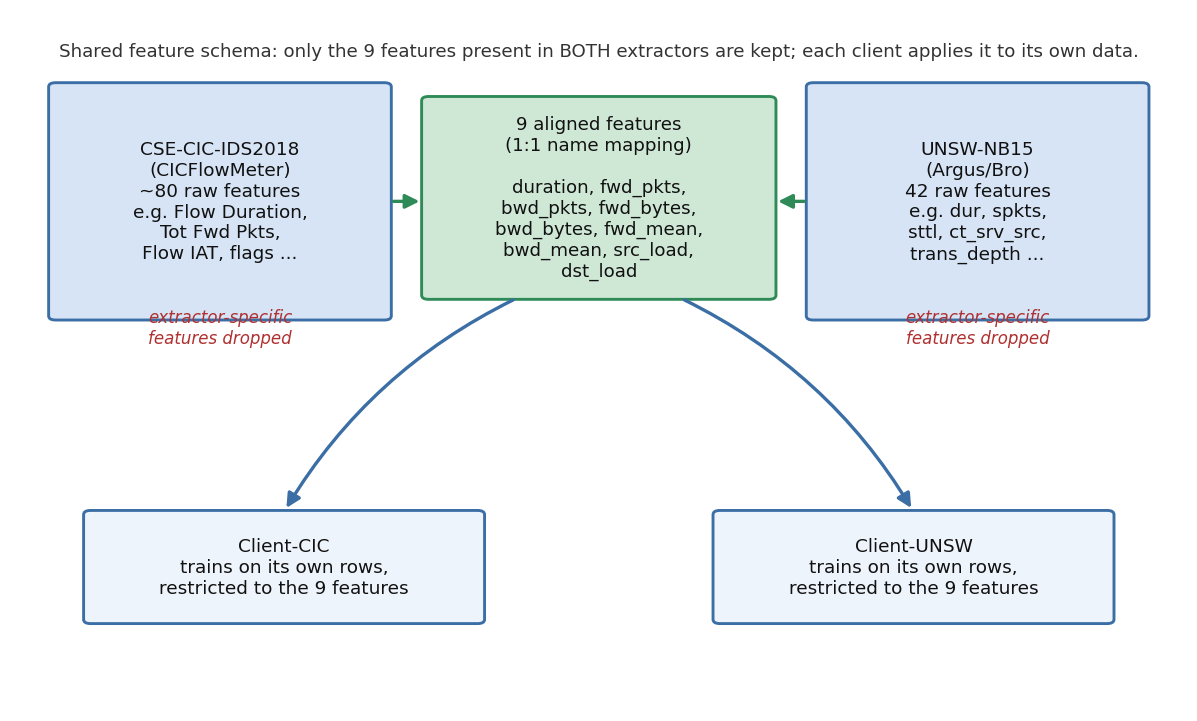
\includegraphics[width=0.62\textwidth]{fig_feature_alignment.png}}
\caption{Far-domain feature alignment (9-feature intersection).}
\label{fig:align}
\end{figure}

\subsection{Federated Architecture}
Our federation follows a horizontal cross-silo pattern with one aggregator and two clients, each
holding one dataset (Fig.~\ref{fig:arch}). Each client trains on its own data and returns only weight
updates; feature normalization (z-score) is computed locally per client, so no data statistics leak
between clients. Each round the aggregator sends the global model, each client trains locally, and the
aggregator combines updates with FedAvg (weighted by data size) for 100 rounds. In the far-domain runs
the three nodes are three \texttt{t3.medium} Amazon EC2 instances exchanging weights via Amazon S3;
the near-domain and non-IID sweeps are run as controlled simulations with identical FedAvg, z-score,
and model code.

\begin{figure}[htbp]
\centerline{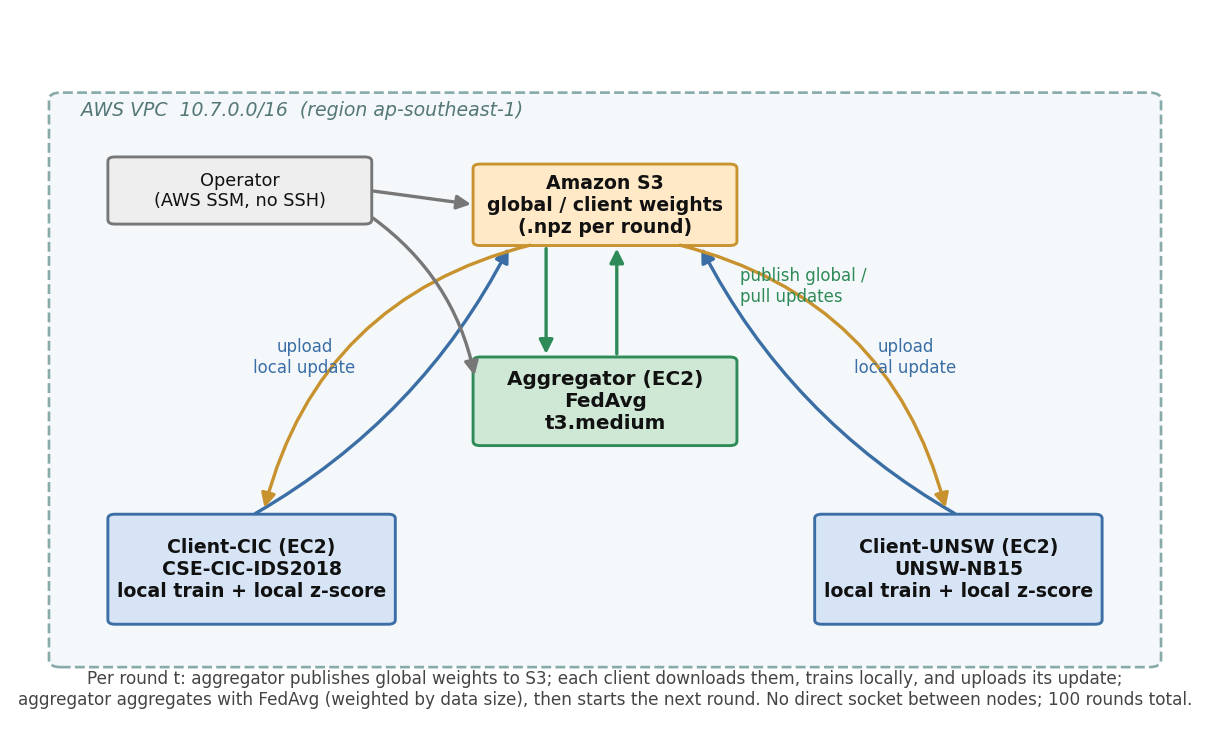
\includegraphics[width=0.58\textwidth]{fig_fl_architecture.png}}
\caption{Federated learning architecture.}
\label{fig:arch}
\end{figure}

\subsection{Model, Metrics, and Claims}
All clients use an identical lightweight multilayer perceptron ($d{\to}128{\to}64{\to}1$ with ReLU
hidden units, sigmoid output, binary cross-entropy loss), trained with mini-batch SGD (batch 256,
learning rate 0.003) for five local epochs per round over 100 rounds; $d$ is 9 (far) or 76 (near).
This shallow MLP is a deliberate \emph{controlled backbone} rather than a performance-maximizing
choice. A small model keeps the per-round payload tiny (about 76.8~KB per client), which is essential
for a cross-silo deployment and is itself the object of the R4 cost measurement; it also isolates the
effects we study---aggregation (FedAvg vs FedProx), non-IID degree, cross-domain transfer, and the
adversarial decision-score shift---from the confounding training dynamics of large, high-capacity
models, such as latent-representation overfitting, whose behavior under federated aggregation is
harder to attribute. Because the architecture is held fixed and identical across all clients and
scenarios, any measured difference is attributable to the factor under test rather than to
model capacity. The primary metric is the Matthews correlation coefficient (MCC), reliable under
class imbalance; we
also report recall and attack success rate (ASR), the share of attacks detected before a perturbation
that evade detection afterwards. We verify six claims: R1 FedAvg vs FedProx; R2 non-IID impact
(Dirichlet $\alpha$ sweep); R3 cross-dataset feasibility; R4 cloud cost; R5 evasion (FGSM, PGD, JSMA);
and R6 adversarial training as a defense. We use five seeds $\{13,42,101,202,303\}$ for R3/R5/R6 and
the near-domain runs, and three seeds for R1/R2, reporting mean and 95\% confidence interval. The data
partition is fixed, so variation reflects training randomness only.

\subsection{Leakage-Free Evaluation Protocol}
A central methodological point is how test data is normalized. In the EC2 federated runs, z-score
statistics are fit per client on its own training split and never shared; to be consistent, each
client's test set is normalized with its owner's training statistics, and results are reported per
client and on the union of both test sets. This is the \emph{leakage-free} protocol. For contrast we
also report a \emph{pooled} evaluation, where all test data is normalized with statistics pooled
across clients; this is internally inconsistent with how the federated model was trained and does not
preserve statistic privacy. The centralized baseline is reported with both pooled and per-domain
(local) normalization, to separate the effect of normalization from the effect of federation. As we
show next, failing to state the evaluation protocol can make the same federated model look like a
failure.

\section{Results}
\label{sec:results}

\subsection{Far-Domain Verification (R1--R6)}
Table~\ref{tab:results} summarizes the six claims in the far-domain configuration.

\begin{table}[htbp]
\caption{Far-domain verification of six FL-NIDS claims.}
\label{tab:results}
\begin{center}
\footnotesize
\begin{tabular}{|l|l|c|}
\hline
\textbf{Claim} & \textbf{Our lab result} & \textbf{Holds?} \\
\hline
R1 FedProx$>$FedAvg & 0.572 vs.\ 0.571, n.s. & No \\
R2 non-IID harms FL & CIC drops; UNSW flat & Domain dep. \\
R3 cross-dataset hard & fed.\ 0.65 vs.\ cen.\ 0.62 & No \\
R4 comm.\ cost & 300 KB, 16 s / round & --- \\
R5 evasion & ASR 0.91 at budget 0.1 & Yes \\
R6 adv.\ training & CIC up; UNSW breaks & Domain dep. \\
\hline
\end{tabular}
\end{center}
\end{table}

\textit{R1 (FedProx vs FedAvg): does not hold.} FedAvg and FedProx are statistically
indistinguishable (MCC 0.572 vs 0.571), both converging in 7--11 rounds.

\textit{R2 (non-IID impact): domain dependent.} On Client-CIC, MCC is stable at high $\alpha$ and
falls to 0.387 at $\alpha{=}0.1$ with a large standard deviation; on Client-UNSW it stays flat or
rises. We attribute this asymmetry mainly to the class balance of the two training sets rather than to
intrinsic separability alone: CIC is strongly benign-skewed (16.9\% attacks), so an extreme Dirichlet
partition can leave some local shards with too few attack samples to learn the minority class,
collapsing and destabilizing the aggregate; UNSW is attack-majority (55.1\%), so even an extreme
partition leaves every shard with a dense-enough attack subset for local convergence. The claim thus
holds for CIC at low $\alpha$ but not for UNSW, with the attack ratio as the plausible driver.

\textit{R3 (cross-dataset FL is hard): does not hold under a consistent protocol.} Under the
leakage-free protocol the federated model reaches a union-test MCC of $0.647 \pm 0.020$ (five seeds;
CIC 0.533, UNSW 0.610). A centralized model reaches $0.565 \pm 0.028$ (pooled norm) and
$0.616 \pm 0.012$ (per-domain norm), so at matched normalization the federated model is slightly but
consistently better (difference $+0.031$, Welch $p{=}0.009$). Single-network (local-only) models fail
to transfer: trained on CIC they reach $0.226$ on the union set, trained on UNSW only $0.010$.
Crucially, the same federated model evaluated with pooled statistics inconsistent with its training
falls to $0.229 \pm 0.228$, erratic across seeds---an evaluation artifact, not a model failure
(Fig.~\ref{fig:results}).

\textit{R4 (cloud cost): measured.} Each client upload is 76.8~KB, so aggregator traffic is about
300~KB per round; 100 rounds take about 27 minutes (about 16 seconds per round including S3 sync).

\textit{R5 (evasion): holds.} We state the threat model explicitly: the attack operates in the
tabular flow-feature space under a white-box assumption, and perturbations are clipped per feature to
its 1st--99th training percentile but are \emph{not} constrained to preserve cross-feature protocol
consistency (for example, changing flow duration without re-deriving the corresponding byte and packet
counts). Our ASR is therefore a measure of \emph{feature-space vulnerability as a worst-case upper
bound}, not of packet-level deliverability; we do not claim the perturbed flows could be transmitted
on the wire. This framing is intentional: it isolates how fragile the learned decision surface is,
independent of the engineering effort an attacker would need to realize such a flow. On a healthy base
(recall 0.61, MCC 0.647), at $\epsilon{=}0.1$ ASR reaches 0.89 (FGSM) and 0.91 (PGD); for
$\epsilon{\geq}0.2$ ASR is at least 0.98 and MCC turns negative. JSMA, changing only two features, is
weaker (ASR 0.37--0.91).

\textit{R6 (adversarial training): domain dependent.} On CIC it helps (MCC under PGD 0.149$\to$0.500,
ASR 0.74$\to$0.13), but on UNSW the clean MCC drops from 0.610 to 0.170 and recall from 0.70 to 0.10.
We explain this in Section~\ref{sec:discuss}.

\begin{figure}[htbp]
\centerline{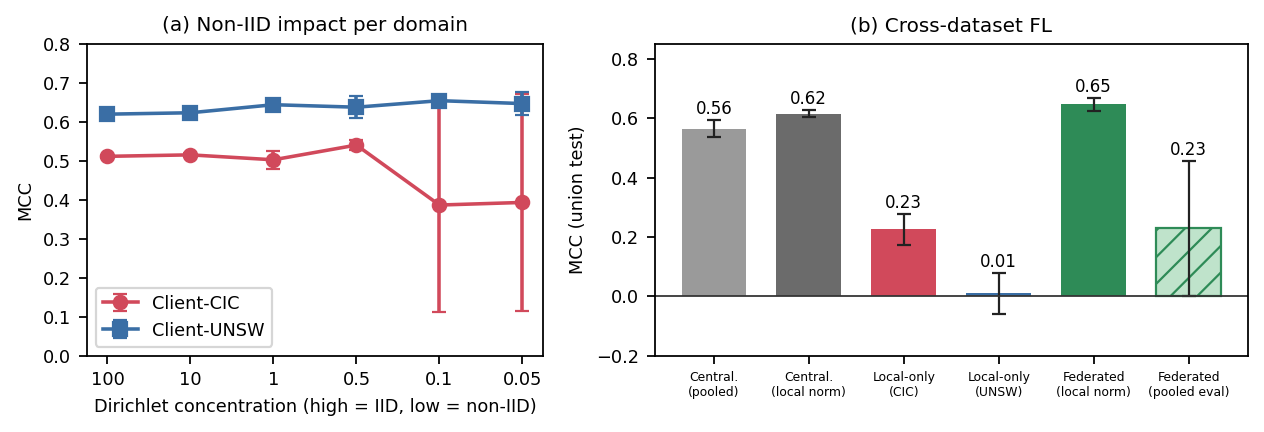
\includegraphics[width=0.75\textwidth]{fig_results.png}}
\caption{Far-domain: (a) non-IID impact differs by domain (R2); (b) cross-dataset FL on the union test
set (R3). Error bars: standard deviation (a), 95\% CI (b).}
\label{fig:results}
\end{figure}

\subsection{Near-Domain: Closer Domains, Richer Features}
When both clients share an extractor (CIC-IDS2017 and CSE-CIC-IDS2018, 76 features), the feature space
is far richer and the attack ratios are similar (19.3\% vs 23.8\%), unlike the far-domain case
(16.9\% vs 55.1\%). Table~\ref{tab:near} reports the partitions and Table~\ref{tab:nearres} the
results, with the same leakage-free protocol.

\begin{table}[htbp]
\caption{Near-domain partitions (CICFlowMeter 2017 vs 2018, 76 features).}
\label{tab:near}
\begin{center}
\footnotesize
\begin{tabular}{|l|c|c|c|}
\hline
\textbf{Client (split)} & \textbf{Total} & \textbf{Attack} & \textbf{Ratio} \\
\hline
CIC2017 (train) & 100{,}000 & 19{,}261 & 0.193 \\
CIC2017 (test)  & 239{,}997 & 46{,}226 & 0.193 \\
CIC2018 (train) & 100{,}000 & 23{,}829 & 0.238 \\
CIC2018 (test)  & 299{,}997 & 71{,}487 & 0.238 \\
\hline
\end{tabular}
\end{center}
\end{table}

The federated model reaches a union-test MCC of $0.851 \pm 0.020$, well above the far-domain value
(0.647) and slightly above the centralized baseline (0.828), while local-only models again fail to
transfer (0.433 and 0.598 on the union set, despite about 0.86 on their own domain). The same
federated model under a pooled evaluation falls to 0.536---the leakage artifact reappears.
Fig.~\ref{fig:near}(a) visualizes this. On non-IID, Fig.~\ref{fig:near}(b) shows both datasets stay
stable down to $\alpha{=}0.5$ and then fall at $\alpha{\leq}0.1$, with variance exploding at the
extreme; the effect is more uniform across datasets than in far-domain.

\begin{table}[htbp]
\caption{Near-domain union-test MCC (mean $\pm$ 95\% CI, five seeds).}
\label{tab:nearres}
\begin{center}
\footnotesize
\begin{tabular}{|l|c|c|c|}
\hline
\textbf{Model} & \textbf{Union} & \textbf{CIC2017} & \textbf{CIC2018} \\
\hline
Federated (local norm) & $\mathbf{0.851 \pm 0.010}$ & 0.895 & 0.821 \\
Centralized (pooled norm) & $0.828 \pm 0.017$ & 0.847 & 0.815 \\
Centralized (local norm) & $0.572 \pm 0.122$ & 0.806 & 0.421 \\
Local-only [CIC2017] & $0.433 \pm 0.085$ & 0.865 & 0.076 \\
Local-only [CIC2018] & $0.598 \pm 0.025$ & 0.047 & 0.837 \\
Federated (pooled eval) & $0.536 \pm 0.038$ & 0.732 & 0.380 \\
\hline
\end{tabular}
\end{center}
\end{table}

\begin{figure}[htbp]
\centerline{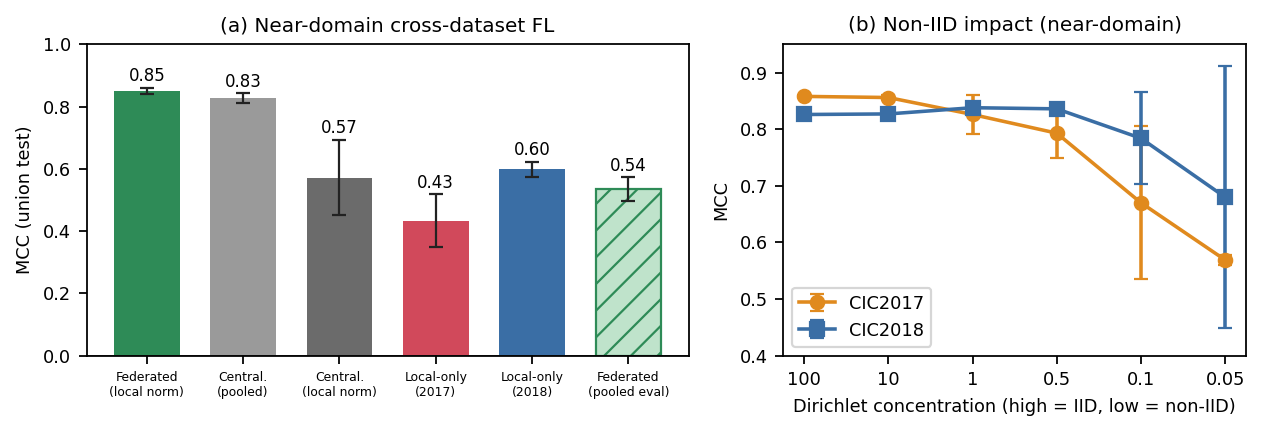
\includegraphics[width=0.72\textwidth]{fig_neardomain.png}}
\caption{Near-domain: (a) federated vs centralized vs local-only on the union test set; (b) non-IID
impact (MCC vs Dirichlet concentration). Error bars: 95\% CI (a), standard deviation (b).}
\label{fig:near}
\end{figure}

\section{Discussion and Threats to Validity}
\label{sec:discuss}

\subsection{Domain-Distance Lesson}
Placed on the domain-distance axis, three lessons are robust. (i) Cross-dataset FL does not collapse;
it \emph{strengthens} as domains get closer (union MCC 0.851 near vs 0.647 far). (ii) Single-network
local-only models always fail to transfer, so federation gives a real benefit at both distances.
(iii) The conclusion is sensitive to the evaluation protocol at both distances: the same federated
model scores 0.65/0.85 under the leakage-free protocol but only 0.23/0.54 under an inconsistent pooled
evaluation. The claim that cross-dataset FL is hard \cite{b5} therefore cannot be assessed without
stating the normalization protocol and a matched baseline.

One confound deserves explicit discussion: the near-domain configuration uses 76 features and the
far-domain one only 9, so part of the 0.65$\to$0.85 improvement could reflect feature count rather
than domain distance. We argue these two factors are not independent but causally linked: the larger
feature space is itself an \emph{inherent consequence} of domain proximity, because both near-domain
clients are produced by the same extractor (CICFlowMeter) and thus share a large, semantically
consistent intersection, whereas the far-domain clients use different extractors (CICFlowMeter vs
Argus/Bro) whose reliable intersection is only nine features. In other words, a richer shared feature
space is precisely what ``closer domain'' means operationally; the two cannot be fully decoupled in
practice. A cleaner isolation would restrict the near-domain clients to the same nine features used in
the far-domain setting and check whether the advantage over far-domain persists; we leave this
feature-controlled ablation as near-term future work, noting that it would attribute the gain to
domain distance net of feature count.

\subsection{Why Adversarial Training Breaks One Domain}
R6 is domain dependent, and we traced the cause by comparing decision-score distributions of the clean
and adversarially trained models over five seeds (Fig.~\ref{fig:advdeg}). Adversarial training shifts
the global decision score uniformly toward ``attack,'' which helps CIC but harms UNSW because the two
domains start from different points. On CIC the mean attack score rises from 0.534 to 0.751, pushing
attacks past the 0.5 threshold and raising recall from 0.48 to 0.91. On UNSW the mean attack score
instead \emph{falls} from 0.687 to 0.325, crossing the threshold the other way, so recall collapses
from 0.70 to 0.10 and the fraction of flows flagged as attacks drops from 0.49 to 0.07. Because FGSM
examples from both clients are aggregated into one global model via FedAvg while each client uses its
own local z-score, the direction that improves CIC opposes the one UNSW needs; the global model cannot
satisfy both and favors CIC, whose attacks are harder to detect. The degradation is thus not random
instability (it is consistent across seeds) but a \emph{cross-domain update-direction conflict under a
static, uniform defense}---direct evidence that domain-aware adversarial defenses are needed in
heterogeneous FL.

\begin{figure}[htbp]
\centerline{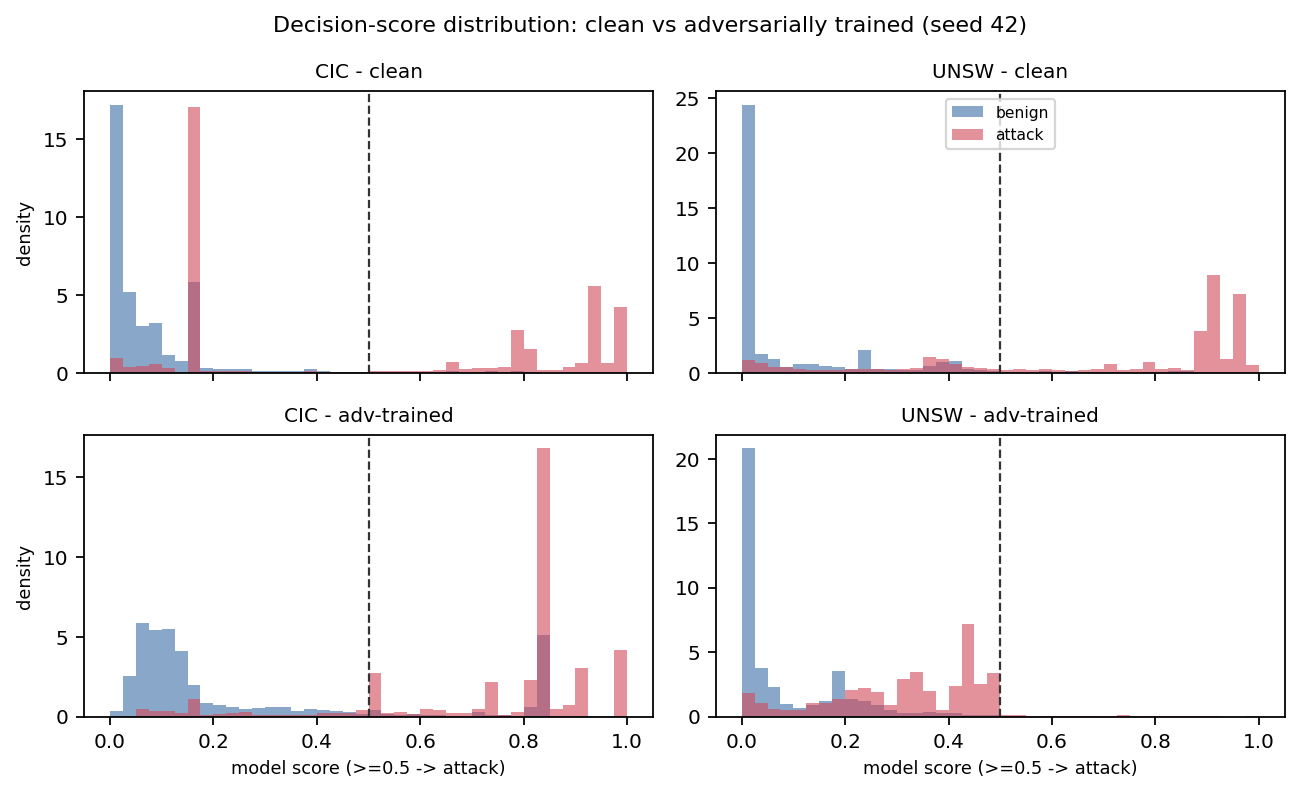
\includegraphics[width=0.72\textwidth]{fig_unsw_degradation.png}}
\caption{Decision-score distributions (benign vs attack), clean vs adversarially trained, per domain.
After adversarial training the UNSW attack scores shift below the 0.5 threshold and are no longer
detected.}
\label{fig:advdeg}
\end{figure}

\subsection{Threats to Validity}
First, we measure whether the \emph{direction} of a claim holds on a uniform testbed, not an exact
replication, so absolute differences from the original papers are expected. Second, the scope is
intentionally narrow: two datasets per configuration and two clients, with three seeds for R1/R2 and
five for the rest; the confidence intervals capture training randomness only, since the partition is
fixed. The decision-score explanation of the UNSW degradation is based on one dataset pair and should
be tested on more pairs. Third, normalization and the evaluation protocol strongly affect results, and
the EC2 (per-client z-score) and simulation (shared global z-score for R1/R2) figures should not be
compared directly. Fourth, the adversarial experiments act on the tabular flow-feature space, not raw
packets, and this is a deliberate scoping choice rather than an oversight: perturbations are clipped
to the 1st--99th percentile of each feature but do not enforce cross-feature protocol or functional
constraints (for instance, byte, packet, and duration relationships), so a perturbed flow need not be
physically realizable on a real network. We therefore interpret the results as a feature-space,
worst-case robustness baseline under a white-box threat model, deliberately separate from
packet-level deliverability; demonstrating that such perturbations can be realized as sendable traffic
is a distinct problem we do not address. Finally, ASR is computed only over attacks detected before
the perturbation and is not comparable across models with different recall.
Fifth, we deliberately fix a single shallow MLP as a controlled backbone (Section~\ref{sec:setup}), so
our findings characterize federated behavior at a fixed, low model capacity; whether the cross-domain
performance gap and the adversarial decision-score shift persist under deeper architectures (for
example 1D-CNN or transformer encoders) is not established here and is left to future work, which
would separate model-capacity limits from genuinely federated effects.

\subsection{Research Directions}
The most pressing directions are standardized, leakage-free normalization and evaluation protocols for
cross-dataset FL; domain-aware evasion defenses instead of static adversarial training; verification of
the reported phenomena under deeper architectures (1D-CNN, transformer) to test whether they are
capacity-independent; semantic-aware feature alignment (which we pursue separately); and validation at
a client and traffic scale closer to production, including IoT traffic domains.

\section{Conclusion}
We studied when cross-dataset federated learning works for network intrusion detection along a
domain-distance axis and under a leakage-free evaluation protocol. Cross-dataset FL does not collapse;
it strengthens as domains get closer (union MCC 0.85 near vs 0.65 far) and consistently beats
single-network models, which fail to transfer. The apparent collapse reported for cross-dataset FL can
be an evaluation artifact: the same federated model falls to 0.23--0.54 when normalized inconsistently
with its training. A healthy model remains highly vulnerable to evasion (ASR 0.91 at budget 0.1), and
adversarial training is domain dependent because it shifts the global decision boundary in a single
direction that cannot serve heterogeneous clients at once---helping one domain while breaking another.
Cloud cost is small (about 300 KB and 16 seconds per round). The main contribution is evidence and
protocol rather than a new method: a reproducible, reasonably priced baseline that shows which FL-NIDS
claims are robust, which are domain dependent, and which are sensitive to the evaluation protocol. All
protocols, scripts, and cloud configurations are released so others can reproduce and build on them.

\begin{thebibliography}{00}
\bibitem{b1} A. Khraisat, A. Alazab, T. Jan, and A. Gopez, ``Survey on federated learning for intrusion detection system,'' \textit{ACM Comput. Surv.}, 2024, doi: 10.1145/3687124.
\bibitem{b2} J. L. Hern\'andez-Ramos \textit{et al.}, ``Intrusion detection based on federated learning: a systematic review,'' \textit{ACM Comput. Surv.}, 2025, doi: 10.1145/3731596.
\bibitem{b3} A. A. Wardana and P. Sukarno, ``Taxonomy and survey of collaborative intrusion detection system using federated learning,'' \textit{ACM Comput. Surv.}, 2024, doi: 10.1145/3701724.
\bibitem{b4} E. V. Fedorchenko, E. Novikova, and A. N. Shulepov, ``Comparative review of the intrusion detection systems based on federated learning,'' \textit{Algorithms}, vol. 15, no. 7, p. 247, 2022, doi: 10.3390/a15070247.
\bibitem{b5} L. Lavaur, Y. Busnel, and F. Autrel, ``Demo: highlighting the limits of federated learning in intrusion detection,'' in \textit{Proc. IEEE ICDCS}, 2024, pp. 1416--1419, doi: 10.1109/ICDCS60910.2024.00135.
\bibitem{b6} J. Zhang \textit{et al.}, ``Combating exacerbated heterogeneity for robust models in federated learning,'' \textit{arXiv:2303.00250}, 2023, doi: 10.48550/arXiv.2303.00250.
\bibitem{b7} S. Saha, M. I. Sayed, M. Faezipour, and S. Bhatt, ``Resilient federated learning for DDoS detection with multi-Krum aggregation,'' in \textit{Proc. IEEE SmartNets}, 2025, doi: 10.1109/SmartNets65254.2025.11106859.
\bibitem{b8} S. Saini, A. Chennamaneni, and B. A. Sawyerr, ``A review of the duality of adversarial learning in network intrusion,'' \textit{arXiv:2412.13880}, 2024, doi: 10.48550/arXiv.2412.13880.
\bibitem{b9} Z. Hu \textit{et al.}, ``Federated meta-learning for few-shot network intrusion detection against advanced persistent threats,'' 2023.
\bibitem{b10} O. Ceviz \textit{et al.}, ``Few-shot federated learning for intrusion detection in UAV networks,'' 2024.
\bibitem{b11} Entente authors, ``Entente: cross-silo federated learning for graph-based NIDS with adaptive contribution scaling,'' 2024.
\bibitem{b12} Y. Chen \textit{et al.}, ``FedAGRU: attention-based federated learning for wireless-edge intrusion detection,'' 2022.
\bibitem{b13} FedIn-NID authors, ``FedIn-NID: dynamic global aggregation for IIoT federated intrusion detection,'' 2023.
\bibitem{b14} R. Doriguzzi-Corin and D. Siracusa, ``FLAD: adaptive federated learning for DDoS attack detection,'' \textit{Comput. Secur.}, 2024.
\bibitem{b15} Resource-efficient FL authors, ``Resource-efficient federated learning for intrusion detection,'' 2023.
\bibitem{b16} Sentinel authors, ``Sentinel: personalized federated learning for heterogeneous intrusion detection,'' 2023.
\bibitem{b17} FedDB authors, ``FedDB: clustering-based federated learning for non-IID intrusion detection,'' 2023.
\bibitem{b18} FedCross-VAN authors, ``FedCross-VAN: feature-alignment federated learning across networks,'' 2023.
\bibitem{b19} Mist-assisted FL authors, ``Mist-assisted hierarchical federated learning for intrusion detection,'' 2022.
\bibitem{b20} IID-vs-non-IID authors, ``An empirical study of IID versus non-IID federated intrusion detection,'' 2022.
\bibitem{b21} S. Ennaji \textit{et al.}, ``Adversarial training for robust federated intrusion detection on Edge-IIoTset,'' 2024.
\bibitem{b22} HADA authors, ``HADA: hardened adversarial defense with SHAP and differential privacy for NIDS,'' 2023.
\bibitem{b23} FedSecIoT authors, ``FedSecIoT: Byzantine-robust federated learning for IoT intrusion detection,'' 2023.
\bibitem{b24} FORT-IDS authors, ``FORT-IDS: outlier-robust aggregation for federated intrusion detection,'' 2024.
\bibitem{b25} GADoT authors, ``GADoT: GAN-based adversarial training for DDoS detection,'' 2022.
\bibitem{b26} Benchmark authors, ``A benchmark of adversarial attacks and defenses for network intrusion detection,'' 2023.
\bibitem{b27} Review authors, ``A review of adversarial robustness in machine-learning intrusion detection,'' 2023.
\bibitem{b28} FeCoGraph authors, ``FeCoGraph: federated graph contrastive learning for intrusion detection,'' 2024.
\bibitem{b29} FedPKT authors, ``FedPKT: prototypical knowledge transfer for federated intrusion detection,'' 2024.
\bibitem{b30} Ensemble+XAI authors, ``An explainable CNN-LSTM-Transformer ensemble for multi-dataset intrusion detection,'' 2023.
\end{thebibliography}

\end{document}
